12. \begin{figure}[ht!]
\center{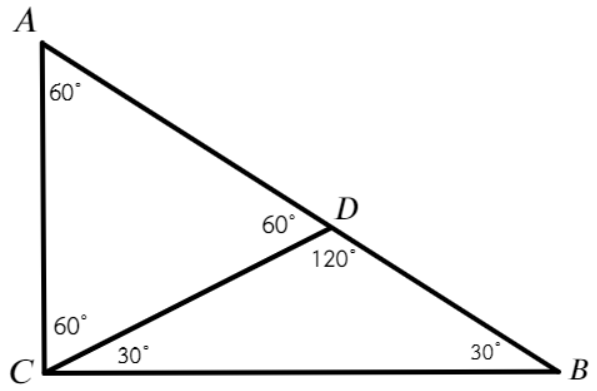
\includegraphics[scale=0.35]{g12.png}}
\end{figure}\\
Треугольник $BCD$ равнобедренный с углом $120^\circ,$ значит углы при основании $BC$ равны $(180^\circ-120^\circ):2=30^\circ.$ Тогда $\angle ACD=\angle C-\angle DCB=90^\circ-30^\circ=60^\circ,\ \angle CAD=180^\circ-\angle C-\angle B=180^\circ-90^\circ-30^\circ=60^\circ,\ \angle CDA=180^\circ-\angle CDB=180^\circ-120^\circ=60^\circ,$
значит треугольник $ACD$ является равносторонним, ч.т.д.\\
